\newpage
\section{Koncepcja i architektura systemu}

\subsection{Założenia projektowe}

Podstawowym założeniem projektowym było przygotowanie rozwiązania, które będzie użyteczne dla użytkownika nietechnicznego przebywającego w domku wypoczynkowym. Asystent głosowy nie powinien pełnić wyłącznie funkcji demonstratora technologii, lecz stanowić intuicyjną warstwę dostępu do informacji zbieranych przez system IoT. Z tego względu za istotne uznano nie tylko poprawne działanie poszczególnych komponentów technicznych, ale również ogólną jakość interakcji, rozumianą jako płynność rozmowy, zrozumiałość odpowiedzi, zgodność z faktami oraz sposób prezentacji informacji w aplikacji.

W procesie projektowym przyjęto, że satysfakcja użytkownika końcowego zależy od wielu powiązanych czynników. Krótki czas odpowiedzi pozostaje ważnym wymaganiem, ponieważ zbyt duże opóźnienie zaburza naturalność rozmowy głosowej. Nie jest to jednak jedyne kryterium oceny systemu. Równie istotne są poprawność języka polskiego, ograniczenie halucynacji modelu, zgodność odpowiedzi z aktualnymi danymi pomiarowymi oraz możliwość przedstawiania informacji w sposób zrozumiały dla osoby, która nie zna struktury systemu technicznego. Z tego powodu projekt zakłada wykorzystanie dynamicznie budowanego kontekstu, który pozwala powiązać odpowiedź modelu z rzeczywistymi odczytami i historią działania domku.

Drugim ważnym założeniem było dostosowanie rozwiązania do ograniczeń urządzenia brzegowego. Przyjęto, że inferencja małego modelu językowego powinna odbywać się lokalnie, na sprzęcie klasy Raspberry Pi 5, co wymaga ostrożnego doboru modeli, parametrów generacji oraz długości przekazywanego kontekstu. W tym sensie projekt ma również charakter badawczy, ponieważ obejmuje sprawdzenie, w jakim stopniu mały model językowy może zostać skonfigurowany tak, aby zapewniał możliwie wysoką jakość odpowiedzi przy ograniczonej mocy obliczeniowej i dostępnej pamięci.

Aby ograniczyć zakres prac niezwiązanych bezpośrednio z głównym problemem badawczym, dla modułów przetwarzania mowy, takich jak detekcja aktywności głosowej (VAD), rozpoznawanie mowy (STT) oraz synteza mowy (TTS), założono wykorzystanie gotowych i zoptymalizowanych rozwiązań. Takie podejście pozwala skoncentrować prace na integracji danych z systemu IoT, mechanizmie budowania kontekstu, architekturze współpracy modeli oraz analizie parametrów wpływających na skuteczność lokalnego asystenta głosowego.

\subsection{Architektura Nauczyciel–Uczeń (Teacher–Student)}\label{subsec:teacher_student}

Zaprojektowane rozwiązanie opiera się na architekturze hybrydowej, w której generowanie odpowiedzi przez model ucznia odbywa się lokalnie na urządzeniu brzegowym (Edge Computing), natomiast przetwarzanie dźwięku oraz zaawansowana analiza danych historycznych realizowane są z wykorzystaniem infrastruktury serwerowej. Takie podejście pozwala ograniczyć obciążenie mikrokomputera znajdującego się w domku, a jednocześnie zachować możliwość badania pracy małego modelu językowego w warunkach ograniczonych zasobów.

Proponowana w pracy architektura Nauczyciel-Uczeń (Teacher-Student) nawiązuje do koncepcji destylacji wiedzy, opisanej w pracy \cite{Hinton2015}. Choć w klasycznym ujęciu oznacza to trening mniejszej sieci na podstawie wyjść sieci większej, w niniejszym projekcie koncepcja ta realizowana jest poprzez hierarchiczne przetwarzanie informacji, model nie poddany kwantyzacji wag ("Nauczyciel") przetwarza surowe dane, przekazując skondensowaną wiedzę modelowi lokalnemu ("Uczniowi").

Serwer pełni rolę "Nauczyciela", wykorzystując moc GPU do okresowego uruchamiania dużego modelu językowego (o wysokiej liczbie parametrów), który jest zbyt wymagający dla urządzenia brzegowego. Model ten analizuje surowe logi z całego dnia i generuje zwięzłe, wysokiej jakości podsumowanie w języku naturalnym. Wygenerowane przez serwer podsumowanie jest przesyłane do domku i służy jako "wiedza wstępna" dla lokalnego asystenta ("Ucznia"). Dzięki temu model na Raspberry Pi nie musi samodzielnie analizować tysięcy rekordów danych, lecz otrzymuje gotową syntezę (np. "Wczoraj zużycie energii było wyższe niż zwykle z powodu włączonej klimatyzacji"), co znacznie podnosi jakość i trafność jego odpowiedzi przy minimalnym obciążeniu procesora.

\subsection{Schemat przepływu danych w systemie}\label{subsec:przeplyw}

\begin{figure}[H]
    \centering 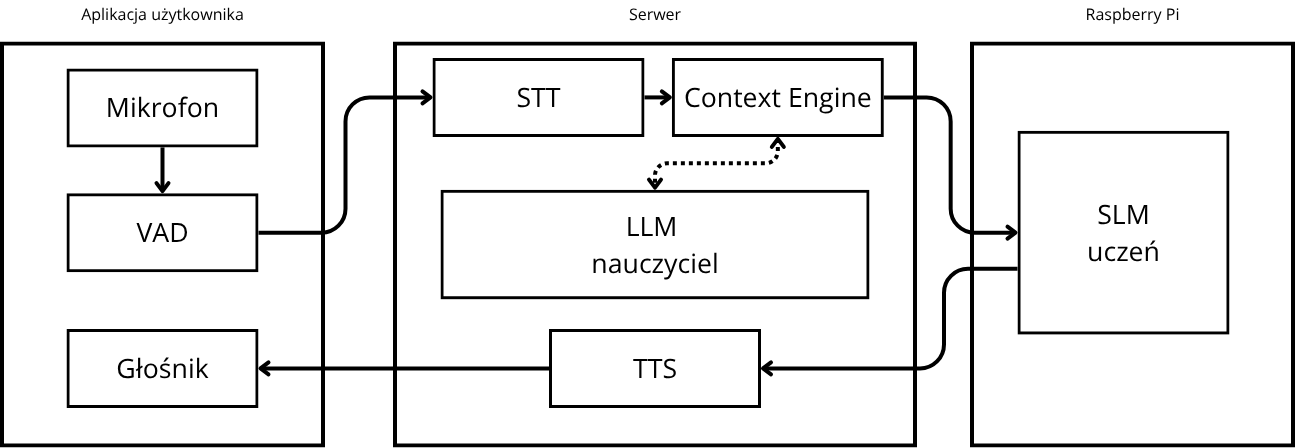
\includegraphics[width=1\linewidth]{src/img/system-schemat.png}
    \caption{Architektura systemu.}
    \label{fig:schemat}
\end{figure}

Przedstawiona architektura zakłada wykorzystanie istniejącej aplikacji użytkownika, rozwijanej wcześniej w ramach systemu Wilga MiLL. W ramach niniejszej pracy nie projektowano aplikacji od podstaw, lecz przyjęto rozszerzenie jej o dodatkową zakładkę asystenta głosowego. Zakładka ta pełni rolę punktu styku pomiędzy użytkownikiem a systemem: umożliwia rozpoczęcie rozmowy, rejestrację wypowiedzi, przekazanie nagrania do dalszego przetwarzania oraz prezentację odpowiedzi w formie tekstowej lub dźwiękowej. Takie podejście pozwala wykorzystać istniejący interfejs, a jednocześnie ogranicza zakres zmian w części aplikacyjnej do funkcji bezpośrednio związanych z asystentem.

W przyjętym rozwiązaniu aplikacja webowa nie realizuje samodzielnie rozpoznawania mowy ani syntezy odpowiedzi. Jej zadaniem jest obsługa interakcji użytkownika oraz przekazanie nagranego sygnału audio do warstwy serwerowej. Po stronie serwera uruchamiane są moduły odpowiedzialne za detekcję aktywności głosowej, transkrypcję mowy na tekst oraz zamianę odpowiedzi tekstowej na dźwięk. Rozdzielenie tych zadań uznano za zasadne, ponieważ pozwala ograniczyć wymagania wobec urządzenia użytkownika oraz skorzystać z większej mocy obliczeniowej dostępnej poza domkiem wypoczynkowym.

Centralnym elementem części badawczej pozostaje mały model językowy, określany jako SLM (Small Language Model), uruchomiony na mikrokomputerze Raspberry Pi. Zdecydowano się wyizolować właśnie ten komponent jako główny element pracujący na sprzęcie o ograniczonych zasobach, ponieważ model językowy stanowi najbardziej wymagającą część całego łańcucha przetwarzania. Raspberry Pi 5 wyposażone w 8 GB pamięci RAM i pozbawione dedykowanej karty graficznej narzuca istotne ograniczenia, dlatego praca koncentruje się na sprawdzeniu, czy pojedynczy lokalny model może generować odpowiedzi o jakości wystarczającej dla użytkownika końcowego.

Drugim modelem w systemie jest większy model językowy, pełniący rolę nauczyciela. Jest on uruchamiany po stronie serwera i odpowiada za przygotowywanie informacji pomocniczych dla modelu ucznia. Jego zadaniem nie jest bezpośrednia obsługa każdej wypowiedzi użytkownika, lecz cykliczna analiza danych oraz tworzenie syntetycznego kontekstu, który może zostać przekazany do małego modelu. Dzięki temu model uruchomiony na Raspberry Pi nie musi samodzielnie analizować pełnych przebiegów czasowych systemu IoT, lecz korzysta z wcześniej przygotowanej reprezentacji wiedzy.

Za koordynację tego procesu odpowiada moduł nazwany Context Engine. W projekcie przyjęto, że jest to zestaw skryptów przygotowanych w języku Python, których zadaniem jest cykliczne pobieranie danych, kierowanie zapytań do modelu nauczyciela oraz budowanie treści wstrzykiwanej następnie do promptu modelu ucznia. Zastosowanie takiego modułu wynika ze sposobu działania modeli językowych, które nie prowadzą samodzielnej, ciągłej analizy środowiska, lecz generują odpowiedź dopiero po otrzymaniu odpowiedniego zapytania. Konieczne było zatem zaprojektowanie warstwy pośredniej, która regularnie przygotowuje kontekst i udostępnia go lokalnemu modelowi w formie możliwej do wykorzystania podczas rozmowy.

Przepływ danych rozpoczyna się od wypowiedzi użytkownika zarejestrowanej w aplikacji webowej. Nagranie jest przekazywane do serwera, gdzie następuje jego przetworzenie do postaci tekstowej. Następnie zapytanie użytkownika zostaje połączone z kontekstem przygotowanym przez Context Engine i przekazane do modelu ucznia uruchomionego na Raspberry Pi. Wygenerowana odpowiedź wraca do warstwy serwerowej, gdzie może zostać przekształcona na mowę, a następnie jest prezentowana użytkownikowi w aplikacji. Taki podział odpowiedzialności pozwala połączyć zalety lokalnej inferencji modelu SLM z możliwościami obliczeniowymi infrastruktury serwerowej.
